%%
%% This is file `sample-acmtog.tex',
%% generated with the docstrip utility.
%%
%% The original source files were:
%%
%% samples.dtx  (with options: `all,journal,bibtex,acmtog')
%% 
%% IMPORTANT NOTICE:
%% 
%% For the copyright see the source file.
%% 
%% Any modified versions of this file must be renamed
%% with new filenames distinct from sample-acmtog.tex.
%% 
%% For distribution of the original source see the terms
%% for copying and modification in the file samples.dtx.
%% 
%% This generated file may be distributed as long as the
%% original source files, as listed above, are part of the
%% same distribution. (The sources need not necessarily be
%% in the same archive or directory.)
%%
%%
%% Commands for TeXCount
%TC:macro \cite [option:text,text]
%TC:macro \citep [option:text,text]
%TC:macro \citet [option:text,text]
%TC:envir table 0 1
%TC:envir table* 0 1
%TC:envir tabular [ignore] word
%TC:envir displaymath 0 word
%TC:envir math 0 word
%TC:envir comment 0 0
%%
%% The first command in your LaTeX source must be the \documentclass
%% command.
%%
%% For submission and review of your manuscript please change the
%% command to \documentclass[manuscript, screen, review]{acmart}.
%%
%% When submitting camera ready or to TAPS, please change the command
%% to \documentclass[sigconf]{acmart} or whichever template is required
%% for your publication.
%%
%%
\documentclass[acmtog]{acmart}
%%
%% \BibTeX command to typeset BibTeX logo in the docs
\AtBeginDocument{%
  \providecommand\BibTeX{{%
    Bib\TeX}}}

%% Rights management information.  This information is sent to you
%% when you complete the rights form.  These commands have SAMPLE
%% values in them; it is your responsibility as an author to replace
%% the commands and values with those provided to you when you
%% complete the rights form.
\setcopyright{acmlicensed}
\copyrightyear{2025}
\acmYear{2025}
\acmDOI{XXXXXXX.XXXXXXX}

%%
%% Submission ID.
%% Use this when submitting an article to a sponsored event. You'll
%% receive a unique submission ID from the organizers
%% of the event, and this ID should be used as the parameter to this command.
%%\acmSubmissionID{123-A56-BU3}

%%
%% For managing citations, it is recommended to use bibliography
%% files in BibTeX format.
%%
%% You can then either use BibTeX with the ACM-Reference-Format style,
%% or BibLaTeX with the acmnumeric or acmauthoryear sytles, that include
%% support for advanced citation of software artefact from the
%% biblatex-software package, also separately available on CTAN.
%%
%% Look at the sample-*-biblatex.tex files for templates showcasing
%% the biblatex styles.
%%

%%
%% The majority of ACM publications use numbered citations and
%% references.  The command \citestyle{authoryear} switches to the
%% "author year" style.
%%
%% If you are preparing content for an event
%% sponsored by ACM SIGGRAPH, you must use the "author year" style of
%% citations and references.
\citestyle{acmauthoryear}


%%
%% end of the preamble, start of the body of the document source.
\begin{document}

%%
%% The "title" command has an optional parameter,
%% allowing the author to define a "short title" to be used in page headers.
\title{Analyzing 5G Network Vulnerabilities with a Forward Look into 6G Security}

%%
%% The "author" command and its associated commands are used to define
%% the authors and their affiliations.
%% Of note is the shared affiliation of the first two authors, and the
%% "authornote" and "authornotemark" commands
%% used to denote shared contribution to the research.

\author{Josue Lopez}
\affiliation{%
  \institution{California Polytechnic State University, San Luis Obispo}
  \city{San Luis Obispo}
  \country{USA}}
\email{jlope424@calpoly.edu}

\author{Noah Giboney}
\affiliation{%
  \institution{California Polytechnic State University, San Luis Obispo}
  \city{San Luis Obisp}
  \country{USA}
}
\email{ngiboney@calpoly.edu}

\author{Peter Kallos}
\affiliation{%
 \institution{California Polytechnic State University, San Luis Obispo}
 \city{San Luis Obisp}
 \country{USA}}
 \email{pkallos@calpoly.edu}


%%
%% By default, the full list of authors will be used in the page
%% headers. Often, this list is too long, and will overlap
%% other information printed in the page headers. This command allows
%% the author to define a more concise list
%% of authors' names for this purpose.
\renewcommand{\shortauthors}{Lopez et al.}

%%
%% The abstract is a short summary of the work to be presented in the
%% article.
\begin{abstract}
  The rapid evolution of wireless communication technologies from 5G to 6G presents both
  unprecedented opportunities and significant security challenges. While 5G enables enhanced
  connectivity, high data rates and support for emerging applications such as autonomous vehicles
  and massive IoT, it also introduces a broader attack surface and increased vulnerability across 
  the network stack. As the research community prepares for the rollout of 6G, new technological 
  and architectural shifts, such as AI-native infrastructure, visible light communication and
  sub-terahertz spectrum use, pose security concerns distinct from those in 5G. This survery paper
  analyzes existing vulnerabilities in 5G networks and investigates how proposed technologies for 6G
  may both mitigate and exacerbate security risks. Our goal is to provide a holistic understanding of
  the wireless network security landscape and to assess how well the 6G paradigm addresses the limitations of its predecessor.
\end{abstract}


%%
%% Keywords. The author(s) should pick words that accurately describe
%% the work being presented. Separate the keywords with commas.
\keywords{5G Security, 6G Networks, Network Vulnerabilities, Wireless  Communication, Cybersecurity, Mobile Network Security}

%%
%% This command processes the author and affiliation and title
%% information and builds the first part of the formatted document.
\maketitle

\section{Introduction}

Wireless communication is changing fast, and with 5G networks now rolling out across the globe, we're seeing incredible advancements like high speed internet, low lag for things like gaming or self-driving cars, and support for highly connected devices like home gadgets. But these improvements come with a catch: 5G networks have a bigger and more complicated attack surface, meaning hackers have more ways to cause trouble. As we look ahead to 6G, the next big step in wireless tech, new features like AI-driven networks, visible light communication, and super-high-frequency bands promise even better performance, but they also bring new security risks that need to be investigated. This survey paper dives into the vulnerabilities of 5G networks and explores how 6G might help some of these issues, while possibly creating new ones in the process. Our goal is to give a clear picture of the security challenges in wireless networks and figure out if 6G is ready to replace 5G networks.

The rise of 5G has brought stellar features like enhanced mobile broadband, ultra-reliable low-latency communication, and massive machine-type communication, which make things like virtual reality and smart cities possible \cite{ref6}. But these advancements rely on technologies like software-defined networking (SDN), network function virtualization (NFV), network slicing, and mobile edge computing (MEC), which open up new weak spots for cyberattacks \cite{ref3}. For example, SDN’s centralized controller can be a single point of failure, and MEC’s distributed setup makes it easier for hackers to target edge devices. Meanwhile, 6G is being designed to push things even further, aiming for extremely fast data speeds and super-low latency for technologies such as holographic calls and high-precision manufacturing \cite{ref4}. But with new features like subterahertz bands and pervasive AI, 6G could introduce risks we haven’t yet seen \cite{ref4_1}.

This paper pulls from key research, like \cite{ref3}, \cite{ref6}, and \cite{ref7} to break down 5G’s strengths and weaknesses, and \cite{ref4} to map out what 6G might look like in the near future. We’ll look at the problems, the technology behind them, and the assumptions researchers make about how these networks plan to operate. The report is organized as follows: Section 2 reviews 5G’s advantages and vulnerabilities. Section 3 explores the shift from 5G to 6G, focusing on new services and technologies. Section 4 digs into 6G’s security enablers, like physical layer security and blockchain, and Section 5 highlights new security challenges 6G might face. Finally, Section 6 provides a conclusion, pointing out where more research is needed to keep 6G secure. Our research aims to provide a clear understanding of both the implementation steps 6G must take in order to avoid the pitfalls of 5G, and the unique challenges 6G will inevitably face. 

\section{Review of 5G Security: Advantages and Vulnerabilities}
The progression of wireless communication standards and next generation data systems tend to provide faster data speeds, lower latency, and greater connectivity among devices. 5G has introduced all these improvements in performance, enabling services such as autonomous vehicles and mobile broadband communications to operate more efficiently and at a much larger scale. With these new capabilities, however, comes a broader and more complex attack surface for malicious actors to exploit. This section covers three of our foundational papers: \cite{ref3}, \cite{ref6}, and \cite{ref7} to showcase 5G's benefits and the security challenges they create.

\subsection{Advantages of 5G Technology}
5G networks deliver enhanced mobile broadband (eMBB), ultra-reliable low-latency communications (uRLLC), and massive machine-type communications (mMTC) \cite{ref6}. These applications are the product of some of the core technologies used in 5G which include software-defined networking (SDN), network function virtualization (NFV), network slicing, and mobile edge computing (MEC). All of them come together to create networks that are efficient, flexible, and dynamic. 

\subsubsection{SDN Advantages} SDN is a network management approach that separates the control plane from the data plane to allow for the centralized control and programmability of network infrastructure. In SDN, a logically centralized controller manages network behavior through standardized protocols like OpenFlow to enable the configuration of network components \cite{ref3}. SDN enhances mobile networks by providing near real-time network control and efficient resource sharing \cite{ref6_1}. It provides an easy way to manage different kinds of hardware, backhaul technologies, and configuration interfaces to enable flexible network connectivity and service provisioning between edge-to-edge networks over various transport systems \cite{ref6_1}. SDN helps solve problems like IP address translation, control signaling overhead, and tunneling by dynamically adjusting traffic flows or tuning codec schemes for wireless links \cite{ref6_1}. Within mobile networks, SDN enables cross-layer coordination between the mobile and transport layers. This allows flow tables in switches and routers to be updated directly without the need to reroute traffic to new switches and routers. This eliminates the need for IP address translation and tunneling which is useful for user mobility in MEC setups \cite{ref6_1}. SDN is what allows 5G to be user-centric, flexible, scalable, achieve high capacity, and provide low latency \cite{ref6}.
\begin{figure}[h]
  \centering
  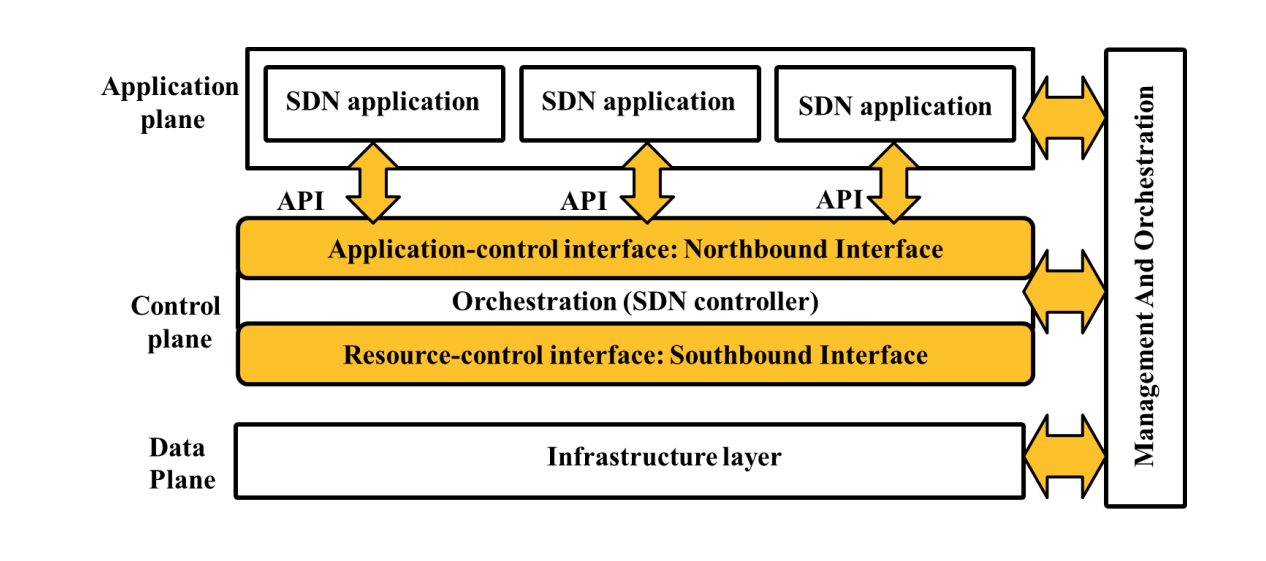
\includegraphics[width=\linewidth]{sdn.png}
  \caption{SDN layered architecture \cite{ref7_1}}
\end{figure}


\subsubsection{NFV Advantages} NFV enhances traditional network operations by virtualizing network services (e.g. routers, firewalls, load balancers) that were historically implemented on dedicated hardware. The software that provide this virtualization are known as virtual network functions (VNFs). Additionally, the NFV infrastructure (NFVI) encompasses hardware and software components like CPUs, storage, and virtualization layers. This provides the environment for VNF deployment. There's also NFV management and orchestration (NFV MANO) which manages the life cycle management of VNFs and the organization of physical and virtual resources within the NFVI \cite{ref6_1}. NFV MANO also handles fault management scenarios like replacing a virtual machine (VM) when it fails, and supports connectivity across MEC platforms deployed in different locations. This can be effective when integrated with SDN for service chaining (linking different network services like firewalls, load balancers, and routers in a specific order to handle network traffic) \cite{ref6_1}. NFV works closely with SDN, complementing it to provide flexibility, scalability, and low latency (but not high capacity) seen in 5G networks \cite{ref6}.
\begin{figure}[h]
  \centering
  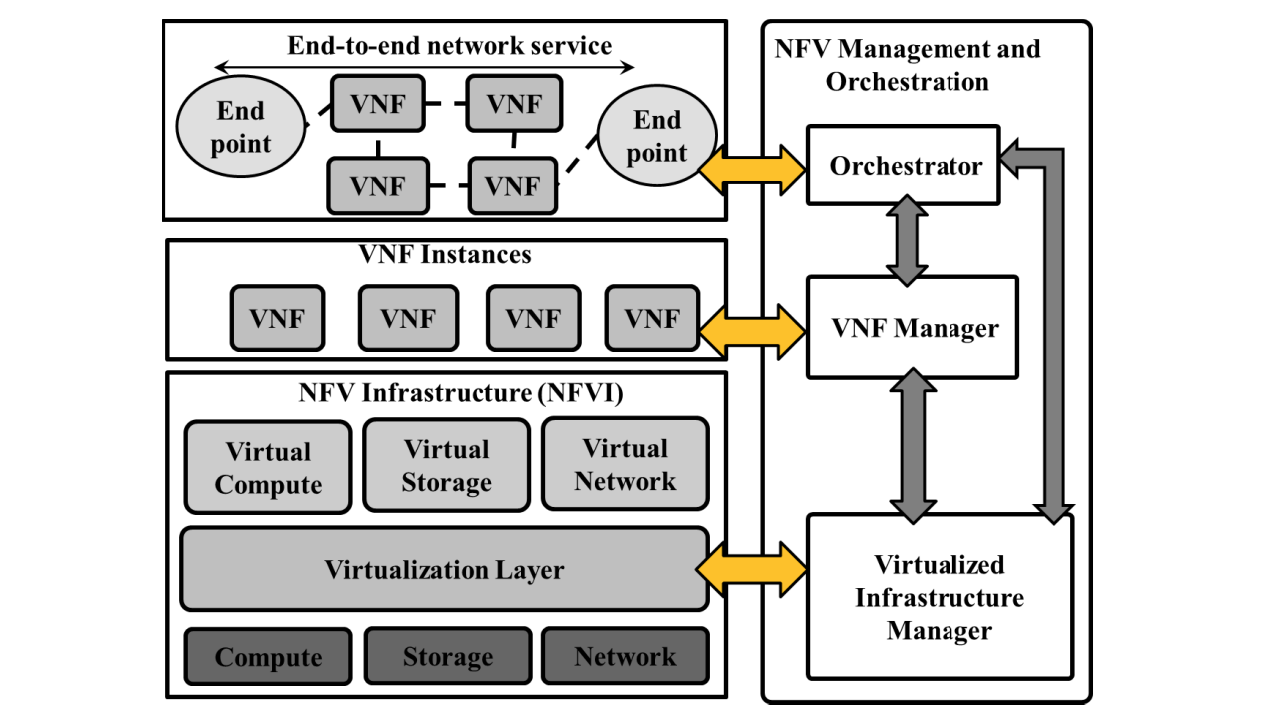
\includegraphics[width=\linewidth]{nfv.png}
  \caption{NFV high level architecture \cite{ref7_1}}
\end{figure}

\subsubsection{Network Slicing Advantages} Network slicing divides a single physical network into various smaller networks known as a network slice. These individual slices can be specialized for a specific type of service or application and can be made of both virtualized and non-virtualized resources \cite{ref7_1}. From an operational perspective, network slicing introduces the concept of a network slice broker, which enhances resource sharing between virtual Mobile Network Operators (MNOs), services, and applications in 3rd Generation Partnership Project (3GPP) mobile networks. This broker complements network sharing management and service exposure capabilities that enables the efficient allocation of resources \cite{ref6_1}. Network slicing ensures high capacity and performance by leveraging MEC to cache content at the edges of a network. This offloads traffic from the mobile backhaul and core network, freeing up bandwidth and increasing data transmission \cite{ref6_1}. For massive IoT deployments, network slicing helps handle scalability challenges by using MEC for local processing and storage and further optimize signaling for large volumes of smaller data transactions. Customizing network slices depends on the integration of NFV and SDN. NFV and SDN work together to coordinate VNF allocation and edge-cloud service provisioning. This ensures flexible and precise control over service delivery \cite{ref6_1}. Dedicated logical networks (network slices) and their relationship to other network components make them a large player in producing the high efficiency found in 5G networks.
\begin{figure}[h]
  \centering
  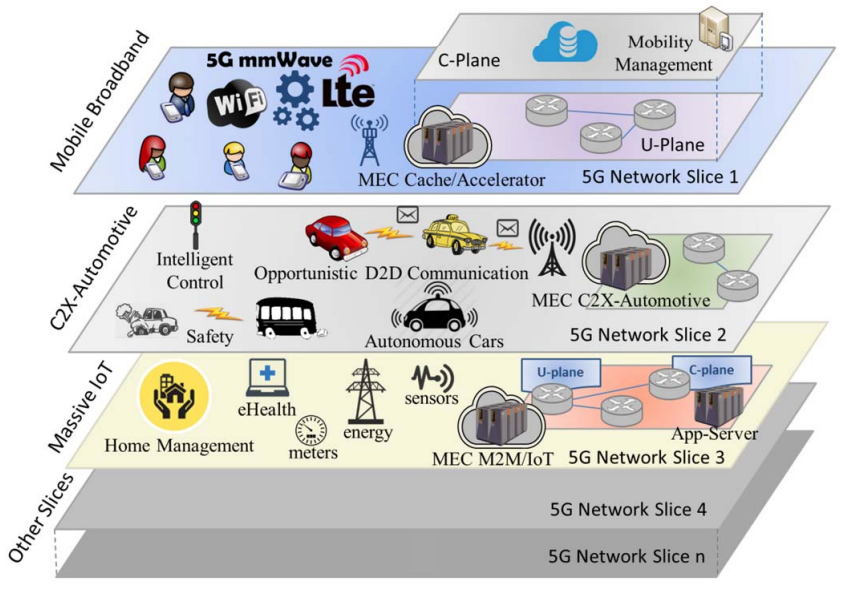
\includegraphics[width=\linewidth]{slice.png}
  \caption{Visualization of network slicing \cite{ref6_1}}
\end{figure}

\subsubsection{MEC Advantages} MEC, also known as multi-access edge computing, is an architecture standard from the European Telecommunications Standards Institute (ETSI) that attempts to shift the geographical location of where data processing occurs to be closer to end-users and their devices. This allows for faster data transmission and reduces the reliance on more distant core networks. The result is ultra-low latency via locally processed data, allowing for useful applications like autonomous driving, augmented reality, and smart city services. \cite{ref6_1} MEC also makes use of the extensive coverage of cellular networks to support machine-to-machine (M2M) communication and general Internet of Things (IoT) applications. MEC, albeit controversially, provides contextual data on user location, preferences, and interests which enables service providers to deliver more personalized experiences \cite{ref6_1}.
\begin{figure}[h]
  \centering
  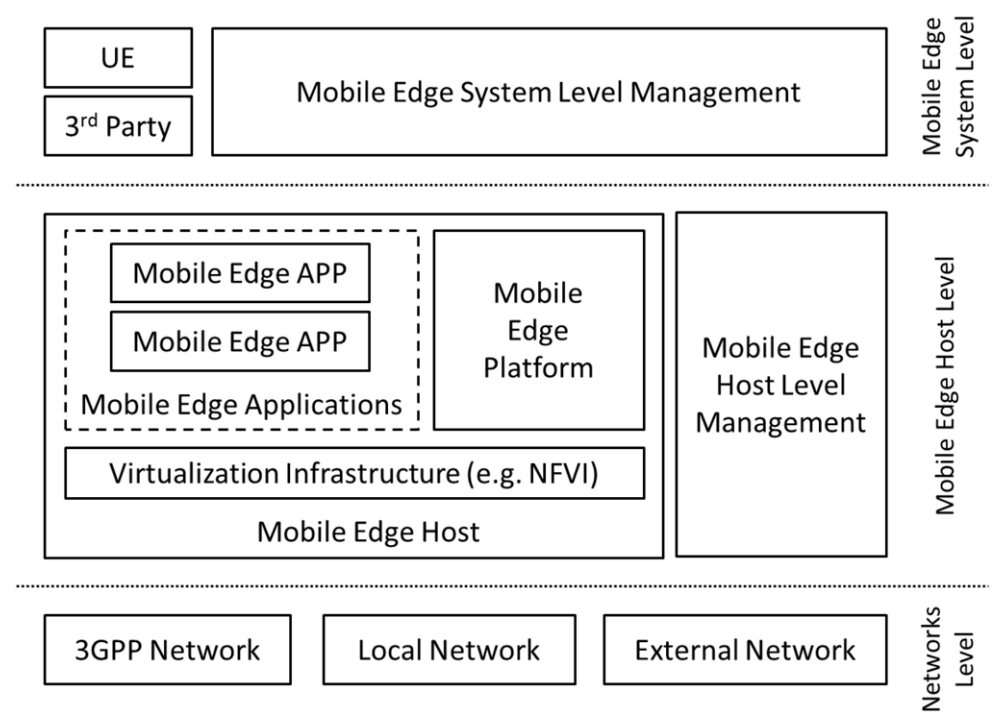
\includegraphics[width=\linewidth]{mec.png}
  \caption{ETSI MEC framework \cite{ref6_1}}
\end{figure}

\subsection{Vulnerabilities Introduced by 5G Advantages}
Although 5G’s use of advanced technologies offers notable benefits, they also create vulnerabilities that expand the attack surface. The following subsections analyze these vulnerabilities and emphasize their flaws.

\subsubsection{SDN Security Challenges}
SDN’s use of a logically centralized controller in the control plane can be a great attack vector due to the device being a single point of failure. All the flow requests, as well as the management and control of data packets, are processed by this centralized controller which makes it an obvious target for attackers. A successful attack on the SDN controller would mean the whole network could be controlled by a bad actor. This would mean the attacker could compromise sensitive information and disrupt entire network operations \cite{ref6}. \cite{Lee05}

A common type of attack that exploits this kind of vulnerability is the distributed denial-of-service (DDoS) attack. Attackers would flood the controller and overwhelm it with a high volume of traffic or control requests. This would exhaust the controller's resources which would primarily disrupt service availability. Smart devices like electricity meters could lose connection to electricity services. This would imply power outages and unstable connections for customers of MNOs and a loss of confidence in these MNOs \cite{ref3}.

\subsubsection{NFV Security Challenges}
NFV relies on a diverse set of hardware providers, virtualization platforms, and VNF developers. This diversity increases the potential weak spots of a network using NFV due to the shared nature of the various components. Each of these components, ranging from physical hardware to virtualized software layers, introduce unique risks. The complexity of managing them all creates opportunities for attackers to exploit misconfigurations and vulnerabilities. 

Hypervisors are essential in running virtualized software and play a critical role in NFV environments. If they are not properly maintained, they can be significant sources of vulnerabilities and potentially allow attackers to compromise VMs and gain unauthorized access to network resources. Attackers can exploit rapid reconfiguration and improperly isolated VNFs to bypass defenses or move through the system and disrupt critical network functions \cite{ref3_1}.

\subsubsection{Network Slicing Vulnerabilities}
The sharing of an infrastructure to create multiple shared networks introduces various security risks related to shared components. Misconfigurations in slice isolation can lead to cross-slice attacks, where a compromised slice can create severe consequences for other slices. Examples include unauthorized access to systems, DoS attacks on neighboring slices, and impersonation attacks. Side-channel attacks are another type of vulnerability that exploit the shared hardware and can result in exposing sensitive data across slices \cite{ref3_2}. The complexity of managing multiple slices increases the likelihood of configuration errors which increases the previously mentioned risks.

 The logical nature of network slices introduces risks in controlling communications across slices. Unprotected or poorly implemented inter-slice user-plane, signaling, or management-plane communications could be disrupted. This would allow attackers to interfere with the services provided by network slices or even initiate unauthorized interactions \cite{ref3_2}. 

Impersonation attacks pose a significant threat, particularly targeting network slice managers or host platforms. A bad actor could impersonate a network slice manager to deploy unauthorized slice instances on physical hosts, or a compromised host platform could falsely present itself as authorized. The potential implications of this are corruption, disclosure, or interruption of services for users \cite{ref3_2}.

\subsubsection{MEC Security Challenges}
The use of a distributed architecture in MEC creates notable security challenges that necessarily complicate security management. The avoidance of going through core networks and the involvement of third-party applications lead to potential billing risks and fraud. Valuable data is transmitted between users and the network edge, meaning the core networks are putting their trust in edge components to handle the sending of users' confidential records, like billing charges, to the home network. Edges of networks are more vulnerable to attack than core networks which creates a large risk of billing errors and fraud. Moreover, edge nodes in networks usually have a lot less computational power and make them great targets for DoS attacks. This can impact the network drastically and spoil the potential of ultra-low latency by degrading it to an unusable state \cite{ref3_3}. 

i want MEC often hosts third-party applications on the same platforms as critical network functions. If these applications are poorly designed or malicious, they can exhaust resources needed by network functions or introduce malware. This could lead to the compromise of the entire platform. In addition, applications have the ability to influence the configuration of the radio access network (RAN), resulting in the DoS of other users \cite{ref3_3}.

\section{Transition from 5G to 6G: Architectural and Technical Changes}

The transition from 5G to 6G networks is driven by the need to address 5G's limitations and enable a new generation of services demanding unprecedented performance levels. This section explores the differences between 5G and 6G, focusing on architectural and technical advancements. The analysis draws heavily from \citet{ref4}, which provides a comprehensive gap analysis of 5G and outlines the vision for 6G. We organize this discussion into three parts: the limitations of 5G necessitating 6G, the new services envisioned for 6G, and the technological enablers defining 6G's architecture.

\subsection{Limitations of 5G}

5G networks have introduced significant advancements over previous generations, enabling services such as enhanced mobile broadband (eMBB), massive machine-type communications (mMTC), and ultra-reliable low-latency communications (URLLC) \citep{ref4}. These services support applications like virtual reality, autonomous driving, and the Internet of Things (IoT). However, 5G struggles to meet the extreme performance requirements of emerging services expected by 2030. According to \citet{ref4}, 5G's architecture, which relies on softwarization, virtualization, millimeter-wave (mm-wave) communications, and massive multiple-input, multiple-output (MIMO), cannot deliver the terabit-per-second data rates, sub-millisecond latencies, and ultra-high reliability needed for future applications. For instance, holographic communications require data rates on the order of terabits per second, which 5G cannot support \citep{ref4_1}. Additionally, 5G's energy efficiency and support for three-dimensional coverage are limited, restricting its ability to handle dynamic, large-scale deployments in scenarios like disaster response or sporadic events \citep{ref4}. These limitations underscore the need for a new generation of wireless networks, driving the development of 6G.

\subsection{New Services Envisioned for 6G}

6G aims to support innovative services that surpass 5G's capabilities, addressing both individual and societal needs. \citet{ref4} identifies several key services that 6G will enable, including:

\begin{itemize}
  \item \textbf{Holographic Communications}: 6G is expected to support immersive 5D communications that integrate all human senses, enabling holographic interactions. These require data rates in the terabit-per-second range, which 5G networks cannot achieve \citep{ref4_1}.
  \item \textbf{High-Precision Manufacturing}: 6G will enhance Industry 4.0 by providing ultra-reliable, low-latency communications (URLLC) with reliability on the order of $1-10^{-9}$ and round-trip latencies of 0.1--1 ms, supporting real-time industrial control with minimal delay jitter \citep{ref4_2}.
  \item \textbf{Sustainable Development and Smart Environments}: 6G will enable pervasive sensing and distributed decision-making for smart cities, intelligent transportation, and energy-efficient systems. This requires 3D communication platforms with near-instantaneous edge cloud functionalities \citep{ref4}.
  \item \textbf{Enhanced Energy Efficiency}: To support sustainable development, 6G aims to achieve communication efficiencies as low as 1 pJ/b, potentially enabling battery-free IoT devices \citep{ref4_3}.
\end{itemize}

These services, summarized in Table \ref{fig:6G_kpi}, demand significant improvements over 5G's key performance indicators (KPIs), such as data rate, latency, reliability, and energy efficiency.

\begin{figure}[h]
  \centering
  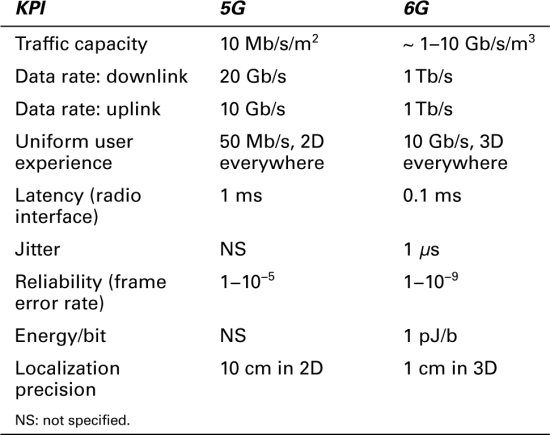
\includegraphics[width=\linewidth]{6G_kpi.png}
  \caption{Comparison of 5G and 6G Key Performance Indicators \cite{ref4}}
\end{figure}

\subsection{Technological Enablers for 6G}

To meet the demanding requirements of these new services, 6G introduces several architectural and technical advancements over 5G. \citet{ref4} highlights the following key enablers:

\begin{itemize}
  \item \textbf{New Architecture}: 6G will feature a new Internet architecture that integrates communication and computation resources. This includes a dynamic data plane for holographic communications, a control plane for nearly deterministic links with low jitter, and a management plane with self-optimization capabilities driven by artificial intelligence (AI) \citep{ref4}.
  \item \textbf{Pervasive AI}: AI will be integral to 6G, enabling self-optimizing networks, semantic communications, and context-aware applications. Semantic communications, which leverage shared knowledge to reconstruct data (e.g., in holographic transmissions), will improve efficiency \citep{ref4_4}.
  \item \textbf{Subterahertz and Visible Light Communications (VLC)}: To support terabit-per-second data rates, 6G will exploit subterahertz bands (90--450 GHz) and VLC. These technologies offer vast bandwidth but require advancements in transceiver and antenna technologies to overcome energy and range limitations \citep{ref4_1}.
  \item \textbf{Energy-Efficient Strategies}: 6G will prioritize energy efficiency through techniques like ambient backscattering and wireless charging, enabling battery-free IoT devices \citep{ref4_5}.
  \item \textbf{3D Coverage}: Unlike 5G's primarily terrestrial infrastructure, 6G will incorporate aerial platforms, such as unmanned aerial vehicles and low-orbit satellites, to provide dynamic, on-demand cloud functionalities in 3D space \citep{ref4}. This is illustrated in Figure \ref{fig:c4_3d_coverage}, which depicts a C4 scenario incorporating 3D coverage.
\end{itemize}

\begin{figure}[h]
  \centering
  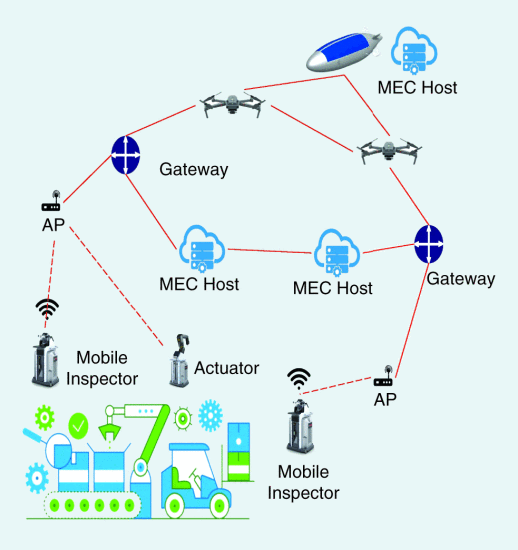
\includegraphics[width=\linewidth]{3D_coverage.png}
  \caption{A C4 scenario incorporating 3D coverage. \cite{ref4}}
\end{figure}

These features collectively address 5G's shortcomings and enable 6G to support next-generation services that will transform society. For instance, the integration of AI and 3D coverage allows 6G to provide near-instantaneous, reliable services in dynamic environments, while subterahertz and VLC technologies meet the high data rate demands of holographic communications.

\subsection{Summary of 5G to 6G Transition}

The transition from 5G to 6G is driven by the need to overcome 5G's limitations in data rate, latency, reliability, and energy efficiency, as well as to support emerging services like holographic communications and high-precision manufacturing. \citet{ref4} provides a clear roadmap for 6G, emphasizing a new architecture, pervasive AI, 3D coverage, and advanced physical layer technologies like subterahertz and VLC. These advancements position 6G to transform industries and societies by enabling a global, intelligent communication infrastructure. A proposed roadmap for 6G development, as outlined in \citet{ref4}, is illustrated in Figure \ref{fig:6g_roadmap}.

\begin{figure}[h]
  \centering
  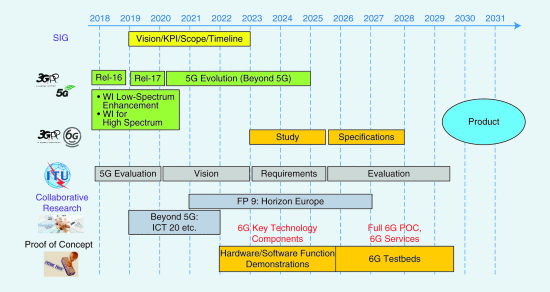
\includegraphics[width=\linewidth]{6G_roadmap.png}
  \caption{A proposed 6G roadmap \cite{ref4}}
\end{figure}

\section{Security Enablers and Issues in 6G Networks}

Before we begin analyzing individual techniques, we first clarify what we mean by a security enabler. An enabler is any architectural feature, protocol primitive, or design paradigm that is built in to a certain technology. Here, we are referring to 6G security enablers specifically, which includes:
\begin{itemize}
  \item \textbf{Lower-layer primitives}: These make attacks physically harder (e.g. beam-level secrecy, secret-key extraction)
  \item \textbf{System-level trust anchors}: These remove single points of failure exposed in SDN/NFV (e.g. verifiable hardware roots, distributed ledgers)
  \item \textbf{Automation levers}: Necessary to keep pace with the speed of machine attacks (e.g. AI driven threat hunting, self healing slices)
  \item \textbf{Post-quantum/context aware cryptography}: Secures the control plane for the lifetime of 6G devices.
\end{itemize}

Each of the following subsections (4.1 - 4.4) examines one enabler through a key reference, then 4.5 summarizes how these enablers connect to the 5G weaknesses cataloged earlier.

\subsection{Enablers Within Physical Layer Security}
\cite{ref1} argue that rethinking security with a "bottom up" approach, from the physical layer, is both viable and efficient for emerging 6G technology. Their survey connects physical layer security techniques with classical cryptography instead of treating them in isolation, and brings forth two physical layer enablers:
\begin{itemize}
  \item \textbf{Secret Key Generation}: Two devices can use the small, reciprocal variations of their shared wireless channel to agree on fresh secret keys every time they connect. \cite{ref1} show that modern short block codes (e.g. Polar or BCH) can reconcile those keys within the allowed latency of uRLLC, although performance can still degrade if an attacker injects well-crafted interference.
  \item \textbf{Device authentication}: \cite{ref1} explores three options. Silicon fingerprints produced by physical unclonable functions (PUF), Location fingerprints for proximity checks, and a combined scheme where a PUF handshake plus the channel-derived key lets devices resume sessions with zero extra round-trips while remaining protected.
\end{itemize}
\cite{ref1} conclude that PLS will not replace higher layer cryptography, but that it will offload part of the trust problem, such as keys, authentication hints, and jamming resilience, onto the physical layer. PLS is treated in this survey as a first line of defense, one which subsequent enablers in higher layers can safely build on.

\subsection{Trust Anchoring: Blockchain and Distributed Ledgers}
Where 4.1 tackled security at the radio link, this subsection moves up above the transport layer, in the distributed control and service management plane of 6G networks. \cite{ref2} propose an answer to the issue of keeping the virtualized, software 6G infrastructure honest: A distributed ledger layer that records every slice and grants resources so that no single SDN controller or NFV manager can be hijacked or spoofed. Specifically, a ledger layer would cover the following capabilities necessary for security within 6G:
\begin{itemize}
  \item \textbf{Tamper proof state}: Slices and edge functions are instantiated, migrated and retired at machine speed. Concrete audit trail left behind.
  \item \textbf{Smart contract automation}:  Full Automation of necessary components for this broker, such as real time spectrum leasing, edge compute brokering and service layer agreement enforcement is entirely possible.
  \item \textbf{Decentralized authentication, authorization and accounting}: Billions of devices can overwhelm central authentication servers. A peer-to-peer ledger spreads the load.
\end{itemize}
\begin{figure}[h]
  \centering
  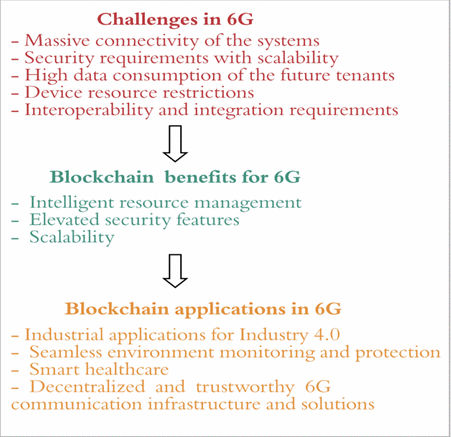
\includegraphics[width=0.8\linewidth,keepaspectratio]{true_ref2_summary.png}
  \caption{Summary of current issues and blockchain solutions \cite{ref2}}
\end{figure}
Combined together, these ledger functions give 6G something that today's 5G stack lacks: a shared source of truth that no operator or attacker can silently rewrite. At the same time \cite{ref2} are clear that a blockchain layer isn't a perfect solution. Reaching appropriate uRLLC targets will force much lighter protocols. Storing petabytes of slice telemetry will require drastic changes, and smart contract bugs as well as quantum vulnerable signatures will open up the system to new attacks. These unresolved issues set the stage for the next two subsections: 4.3 on AI-driven, self healing security operations that can react faster than humans, and 4.4 on post-quantum and context aware cryptography that must protect the ledger's signatures for the lifetime of 6G devices.

\subsection{Security Automation and Adaptivity}
This section continues within the 6G management plane.  \cite{ref5} lay out a research agenda where embedded trust models, AI security automation, and post-quantum cryptography form the next set of security enablers. The authors state that 6G is expected to handle 100 billion devices, 10 times more than 5G, and therefore inherited 5G threats such as botnets and denial of service attacks will scale by an order of magnitude as well. A proposed solution to this is an end-to-end trust model with stable device IDs, cross-domain reputation, and policy driven decisions so that the network itself can reduce risky flows, all boosted by the power of machine learning and artificial intelligence. Some of the core capabilities mentioned in the paper are:
\begin{itemize}
  \item \textbf{Embedded trust networking}: Stable device IDs, cross-domain reputation and policy driven flow admission would let the infrastructure itself refuse suspicious traffic. This would assist in mitigating the SDN-controller denial of service attacks mentioned in Section 2.
  \item \textbf{AI-driven security operations}: Packet-level machine learning would detect and react faster than humans. Works well with PLS and blockchain events mentioned in Sections 4.1 and 4.2, respectively, as ML could be trained with such data.
  \item \textbf{Post-quantum ready cryptography architecture}:  Moving SIM-style credentials and TLS cores to lattice based schemes before quantum attacks arrive would provide a long-lived cryptographic anchor that protects the ledger signatures mentioned in Section 4.2.
\end{itemize}
\begin{figure}[h]
  \centering
  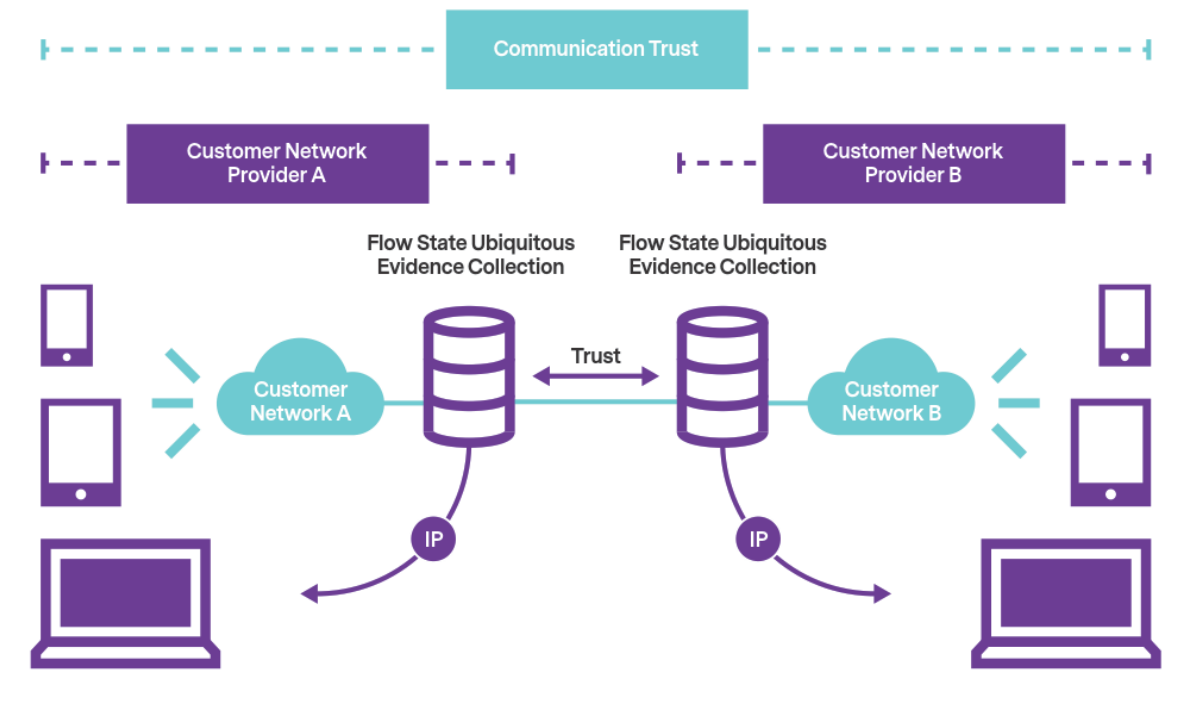
\includegraphics[width=\linewidth]{4.3_1.png}
  \caption{Conceptual model and ID/locator split for trust networking \cite{ref5}}
\end{figure}
\begin{figure}[h]
  \centering
  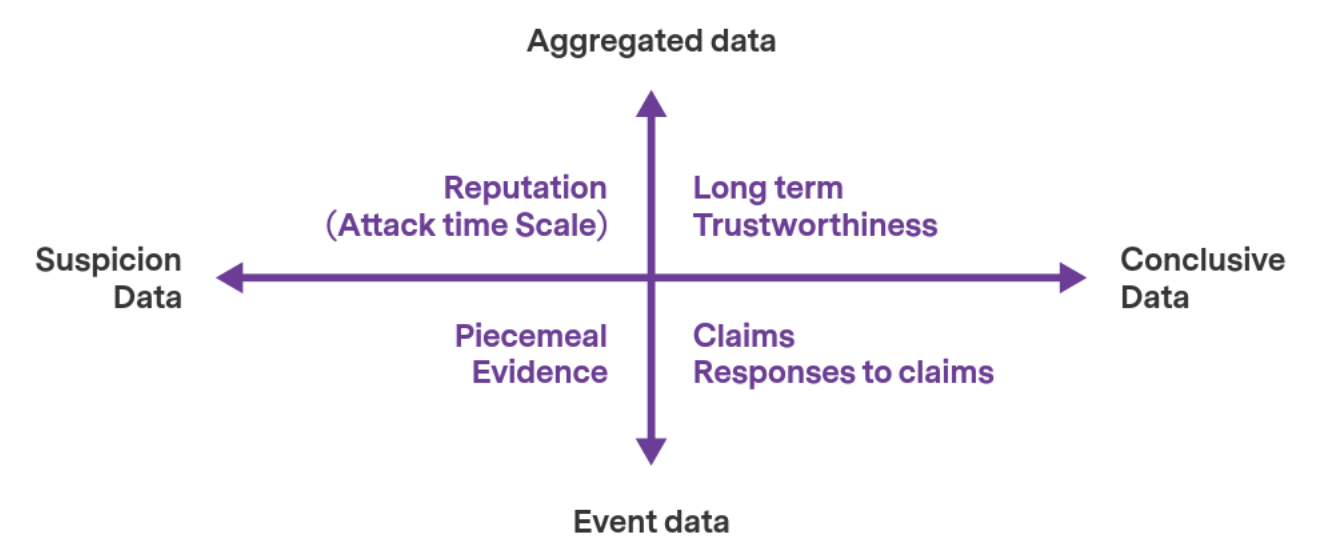
\includegraphics[width=\linewidth]{4.3_2.png}
  \caption{Trust-related data sharing for reputation generation \cite{ref5}}
\end{figure}
Taken together, these automation changes turn security from a static perimeter into a living control loop. One that can raise or lower its defenses as necessary without the need for human reaction. Yet, \cite{ref5} emphasize that the same ingredients produce new risks: New types of ML poisonings that affect reputation scores, policy conflicts between administrative domains, and the performance requirements for such a living, breathing system.

\subsection{Cryptography for a Stable and Secure Future}
Where Sections 4.1 - 4.3 focus on hardening the physical layer, anchoring trust with a ledger, and automating defense with AI respectively, this section turns to the necessary cryptographic and privacy toolkit that must keep those layers trustworthy well into the future, long after quantum computers arrive. \cite{ref8} argue that 6G therefore needs more security enablers, some of which include:
\begin{itemize}
  \item \textbf{Quantum-safe Cryptography}: RSA, ECC, and the blockchain signatures of Section 4.2 all fall to Shor's algorithm once a general purpose quantum computer is built. We must move authentication and key exchanges to a NIST-class lattice, code, or multivariate schemes. 
  \item \textbf{Heterogeneous Cloud Trust Anchors}: In 6G the "cloud" is no longer one large datacenter. It is a continuous web of smaller networks. This flexibility gives us ultra low latency and energy savings, but it also widens the attack surface. \cite{ref8} mention tamper-resistant hardware roots such as TPM 2.0 and DICE chips or similar secured elements as a solution, as well as trusted execution environments.
\end{itemize}
\begin{figure}[h]
  \centering
  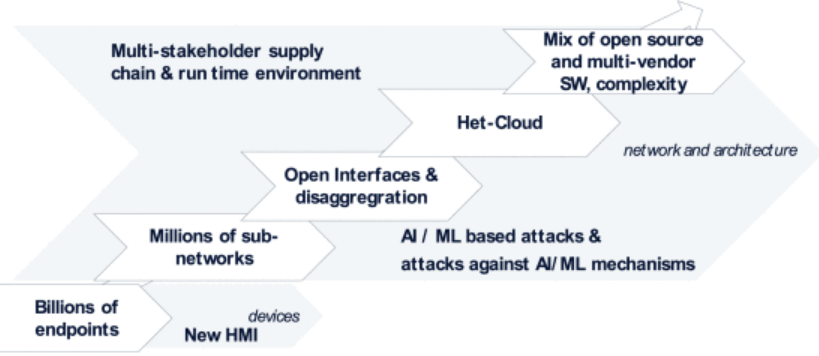
\includegraphics[width=\linewidth]{4.4.png}
  \caption{Heterogeneous cloud technology expands the 6G threat vector \cite{ref8}}
\end{figure}
Together, hardware anchoring and quantum safe algorithms will provide a secure backbone for 6G's existence.

\section{Security Issues Within 6G}
Section 4 showed how the four enablers (physical layer security enhancements, distributed ledger, AI automation, quantum-safe cryptography and heterogeneous cloud trust anchors) provide solutions to the most obvious issues with 5G technology. Respectively, they provide:
\begin{itemize}
  \item \textbf{Per packet origin authentication and fresh keys} 
  \item \textbf{An immutable source of truth for network events} 
  \item \textbf{Machine speed detection and response} 
  \item \textbf{Tamper resistant hardware roots} 
  \item \textbf{Cryptography that would survive the post-quantum world} 
\end{itemize}
These techniques do not form a complete 6G security stack. Instead, they illustrate how different layers could be hardened where 5G is soft. The rest of this section looks at what still breaks, whether that is because the fixes above would have side effects, or because 6G introduces brand new attack surfaces.

\subsection{Scalability and Governing Policy Gaps}
\begin{itemize}
  \item \textbf{Ledger latency}: A slice state blockchain that logs everything will hit petabytes extremely fast. Lightweight solutions/enhancements may come up but might require re-introducing trust into the system, particularly in whoever curates the history.
  \item \textbf{Multi-domain Policy conflicts}: AI driven trust engines can drop traffic that violates their policy, while a neighboring engine might consider that traffic valid. No standardization exists today.
\end{itemize}

\subsection{Machine Learning Issues}
Attackers or adversaries can nudge reputation scores, silently tilting the model. Methods such as mandated and regulated training could slow, but not eliminate, this risk. Models would be trained on new types of data, which also broadens the attack vector. AI must necessarily be regulated and inspected frequently to ensure accuracy, both functionally and ethically.

\subsection{Post-Quantum Transitional Issues}
Lattice or code based key exchanges add more overhead per handshake, which may drastically impact less powerful IoT devices. Some devices are deployed for 20+ years, and rolling out new firmware, certificates, and trust roots before large scale quantum machines arrive remains a heavy task.

\subsection{Takeaways}
The enablers of Section 4 plug critical holes in 5G technology, but 6G's grand scale and autonomy introduce new risks. Scale straining, machine learning issues, and quantum safe solutions that introduce friction all highlight where additional research and governance is still needed.

\section{Conclusion}

In this survey, we explored the security landscape of 5G networks and looked ahead to the potential of 6G, focusing on both the strengths and weaknesses of these technologies. In Section 2, we broke down 5G’s key features, like software-defined networking (SDN), network function virtualization (NFV), network slicing, and mobile edge computing (MEC), and how they make 5G fast, flexible, and scalable \cite{ref6}. We also saw how these technologies create new vulnerabilities. For example SDN’s single point of failure in its controller or MEC’s exposure to attacks at the network edge \cite{ref3}. Section 3 outlined the shift to 6G, highlighting its goals of supporting fast data rates, low latency, and new services like holographic communications and high-precision manufacturing \cite{ref4}. In Section 4, we dug into 6G’s security enablers, such as physical layer security, blockchain for trust, AI-driven defenses, and quantum-safe cryptography, which aim to fix 5G’s weaknesses \cite{ref1,ref2,ref5,ref8}. Finally, Section 5 showed that while 6G’s enablers are promising, they bring new challenges, like blockchain scalability issues, AI model vulnerabilities, and the complexity of transitioning to quantum-safe systems.

Althoug 6G has the potential to address 5G’s security gaps, it’s clear that no single fix will make wireless networks completely secure. The enablers we discussed—like secret key generation, distributed ledgers, and AI-driven threat detection—offer strong defenses against attacks like DDoS or impersonation that are hindering 5G \cite{ref1,ref2,ref5}. But 6G’s massive scale, with billions of connected devices, and its reliance on new tech like subterahertz bands and pervasive AI, create new risks that need more research \cite{ref4}. For example, blockchain ledgers could slow down under the weight of massive data, and AI models could be tricked by clever attackers, messing up trust systems. Moving to quantum-safe cryptography is tough for low-power IoT devices that might stick around for decades.

To make 6G truly secure, the research community needs to tackle these gaps. Here are some key directions in focus for the future:
\begin{itemize}
  \item \textbf{Scalable Security Solutions}: We need lightweight blockchain protocols that can handle 6G’s massive data without slowing down or reintroducing trust issues \cite{ref2}.
  \item \textbf{Robust AI Defenses}: AI-driven security is awesome but risky if models get poisoned. Research should focus on regulated, transparent AI training to keep systems accurate and ethical \cite{ref5}.
  \item \textbf{Quantum-Safe Transition Plans}: Moving to quantum-safe cryptography is critical, but we need practical ways to update long-lasting IoT devices without breaking the bank or their performance \cite{ref8}.
  \item \textbf{Real-World Testing}: Many 6G security ideas sound great on paper but haven’t been tested in realistic network setups. Open platforms for simulating large-scale 6G networks could help researchers validate their solutions \cite{ref4}.
\end{itemize}
This survey shows that while 6G has big plans to fix 5G’s security problems. By studying 5G’s weaknesses and 6G’s proposed solutions, we’ve highlighted what’s working and where we need to go next to keep future of wireless networks safe.

\bibliographystyle{ACM-Reference-Format}
\bibliography{main}

\end{document}
\endinput
%%
%% End of file `sample-acmtog.tex'.
